%% ============================================================
%%  QKD Multi-Protocol Simulator — IEEE Journal-Quality Paper
%%  Author   : Anuj Rathore  |  IIIT Sri City, Chittoor, India
%%  Compiler : pdflatex (two passes) or latexmk -pdf
%%  Notes    : Images assumed in ./assets/  (5 figures from ZIP)
%% ============================================================
\documentclass[journal]{IEEEtran}

%% ---------- Core Packages ----------
\usepackage{cite}
\usepackage{amsmath,amssymb,amsfonts}
\usepackage[T1]{fontenc}
\usepackage[utf8]{inputenc}
\usepackage[final]{graphicx}
\usepackage{booktabs}
\usepackage{array}
\usepackage{tabularx}
\usepackage{multirow}
\usepackage{adjustbox}
\usepackage{url}
\usepackage{hyperref}
\usepackage{xcolor}
\usepackage{listings}
\usepackage{stfloats}
\usepackage{placeins}
\usepackage{microtype}
\usepackage{balance}
\usepackage{algorithm}
\usepackage{algpseudocode}

%% ---------- Graphics path ----------
\graphicspath{{assets/}}
\DeclareGraphicsExtensions{.png,.jpg,.jpeg,.pdf}
\setkeys{Gin}{draft=false}

%% ---------- Listings style ----------
\lstdefinestyle{qkdcode}{
    basicstyle=\ttfamily\scriptsize,
    keywordstyle=\color{blue!70!black},
    commentstyle=\color{gray},
    stringstyle=\color{teal},
    numberstyle=\tiny\color{gray},
    numbers=left,
    stepnumber=1,
    numbersep=5pt,
    breaklines=true,
    breakatwhitespace=true,
    columns=fullflexible,
    keepspaces=true,
    showstringspaces=false,
    frame=single,
    rulecolor=\color{black!30},
    backgroundcolor=\color{gray!5}
}

%% ---------- Hyperref setup ----------
\hypersetup{
  colorlinks=true,
  linkcolor=blue!60!black,
  citecolor=blue!50!black,
  urlcolor=blue!70!black
}

%% ============================================================
\begin{document}
%% ============================================================

\title{A Multi-Protocol Quantum Key Distribution Simulator with\\
Hybrid Desktop-Web Architecture: Design, Implementation,\\
and Rigorous Statistical Evaluation}

\author{%
  \IEEEauthorblockN{Dr. Kartick Sutradhar, Anuj Rathore}
  \IEEEauthorblockA{%
    Department of Computer Science and Engineering\\
    Indian Institute of Information Technology, Sri City\\
    Chittoor, Andhra Pradesh, India\\
    \texttt{anujrathore385@gmail.com}}
}

\markboth{IEEE Transactions on Quantum Engineering,~Vol.~XX,~No.~X,~2025}%
         {Rathore: Multi-Protocol QKD Simulator with Hybrid Architecture}

\maketitle

%% ============================================================
\begin{abstract}
Quantum Key Distribution (QKD) offers provably secure key establishment
grounded in the laws of quantum mechanics, yet practical access to
photonic testbeds remains limited, and existing software tools are
predominantly single-protocol and lack consistent impairment modeling.
This paper presents a unified, open-architecture QKD simulator that
implements four canonical protocols—BB84, B92, E91, and BBM92—within a
single, coherent Python/Qiskit simulation core. The platform models
realistic channel and device impairments, including fiber attenuation,
source and detector inefficiencies, state-of-polarization (SOP)
deviations, and configurable eavesdropping modes. To support diverse
usage patterns, the system exposes both a local desktop interface built
on Tkinter and Matplotlib and a distributed web interface built on
React, Node.js/Express, and a Python bridge, with both frontends sharing
the same simulation backend. Statistical rigor is enforced by a
repeated-run evaluation framework that reports mean, standard deviation,
and 95\% confidence intervals for all key metrics. Across 20 baseline
runs at 10,000 qubits per run, BB84 achieved the highest mean key-rate
estimate of $160{,}045.15 \pm 0.00$~Hz at 25~km, while the E91
Bell-correlation diagnostic yielded a mean CHSH $S$-statistic of
$2.12$, falling to $1.58$ under eavesdropping activation. The simulator
is suitable for academic instruction in quantum cryptography, rigorous
protocol-level benchmarking, and pre-deployment design-space
exploration.
\end{abstract}

\begin{IEEEkeywords}
quantum key distribution, BB84, B92, E91, BBM92, Qiskit, quantum
cryptography, simulator, QBER, Bell inequality, CHSH inequality,
cybersecurity education, hybrid architecture
\end{IEEEkeywords}

%% ============================================================
\section{Introduction}
\label{sec:intro}
%% ============================================================

The advent of large-scale quantum computers poses an existential threat
to classical public-key cryptographic systems such as RSA and
elliptic-curve Diffie-Hellman, whose security rests on the presumed
computational hardness of integer factorization and discrete logarithms.
Shor's algorithm~\cite{shor1994} reduces both problems to polynomial
time on a sufficiently powerful quantum machine, rendering long-lived
classical key infrastructure fundamentally insecure in a post-quantum
era. QKD provides a principled response: rather than basing security on
unproven complexity-theoretic assumptions, it derives security directly
from quantum mechanical principles—specifically, the
no-cloning theorem and the disturbance-inducing nature of quantum
measurement~\cite{lo2014}.

Despite its theoretical appeal, practical adoption of QKD is constrained
by three structural barriers. First, photonic hardware—entangled-photon
sources, single-photon detectors, and fiber-coupled interferometers—is
expensive, fragile, and confined to specialized laboratories. This limits
hands-on experimentation to a small community of researchers.
Second, most publicly available QKD software tools are
protocol-specific: they implement a single protocol in isolation and
expose limited or no facility for systematic comparison under consistent
physical assumptions. Third, statistical reporting in QKD simulation
literature is frequently inadequate, with results drawn from single
runs of inherently stochastic systems, making reproducibility and
reviewer confidence difficult to establish.

This paper addresses all three barriers through a unified, open-source
QKD simulation platform. The contributions of this work are:

\begin{enumerate}
  \item A single simulation core implementing BB84~\cite{bb84},
        B92~\cite{b92}, E91~\cite{e91}, and BBM92~\cite{bbm92} with
        protocol-specific sifting and measurement logic, built on
        IBM Qiskit~\cite{qiskit}.

  \item A physically motivated impairment model incorporating combined
        source-fiber-detector efficiency, SOP angular perturbations,
        stochastic channel noise, and intercept-resend eavesdropping
        toggles.

  \item A hybrid deployment architecture exposing identical simulation
        semantics through a local desktop GUI (Tkinter + Matplotlib) and
        a browser-accessible web application (React + Node.js/Express +
        Python bridge).

  \item A rigorous statistical evaluation framework that employs
        repeated runs with mean, standard deviation, and bootstrap-style
        confidence interval reporting for all numerical claims.

  \item Comprehensive sensitivity analysis over fiber length and
        protocol parameters, demonstrating the utility of the platform
        for pre-deployment design-space exploration.
\end{enumerate}

The remainder of this paper is organized as follows.
Section~\ref{sec:background} provides theoretical background on QKD
protocols. Section~\ref{sec:related} reviews related work.
Section~\ref{sec:architecture} describes the system architecture.
Section~\ref{sec:math} presents the mathematical model.
Section~\ref{sec:implementation} covers the implementation details.
Section~\ref{sec:methodology} specifies the experimental methodology.
Section~\ref{sec:results} presents and analyzes results.
Section~\ref{sec:discussion} discusses implications and threats to
validity. Section~\ref{sec:conclusion} concludes the paper, and
Section~\ref{sec:futurework} outlines directions for future work.

%% ============================================================
\section{Theoretical Background}
\label{sec:background}
%% ============================================================

\subsection{BB84 Protocol}

The BB84 protocol, introduced by Bennett and Brassard in
1984~\cite{bb84}, is the seminal prepare-and-measure QKD scheme.
Alice encodes each random key bit into one of two conjugate bases:
the rectilinear basis $\{|0\rangle, |1\rangle\}$ and the diagonal
basis $\{|+\rangle, |-\rangle\}$. Bob independently and randomly
selects a measurement basis for each received qubit. After transmission,
Alice and Bob publicly announce their basis choices, retaining only
the bits where their bases matched (the \emph{sifting} step). Security
is guaranteed because any eavesdropper (Eve) who measures the quantum
channel must inevitably disturb the state—introducing detectable errors
in the Quantum Bit Error Rate (QBER). If QBER exceeds a threshold of
approximately 11\%, the protocol is aborted.

\subsection{B92 Protocol}

Bennett's 1992 two-state protocol~\cite{b92} reduces the quantum
alphabet to two non-orthogonal states: $|0\rangle$ and $|+\rangle$,
encoding bit 0 and bit 1 respectively. Bob applies one of two
measurement operators; an inconclusive result in either measurement
guarantees that the transmitted state is known, enabling key
extraction. B92 offers a simpler hardware implementation than BB84 but
at the cost of a lower sifting efficiency (approximately 25\% vs.\ 50\%
for BB84), resulting in roughly one-quarter the raw key rate under
comparable channel conditions.

\subsection{E91 Protocol}

Ekert's 1991 protocol~\cite{e91} departs fundamentally from
prepare-and-measure approaches by leveraging Einstein-Podolsky-Rosen
(EPR) entangled photon pairs. A source distributes entangled qubit
pairs to Alice and Bob, each of whom independently selects from a set
of measurement angles. Correlations in their outcomes violate the
CHSH-Bell inequality~\cite{clauser1969}:
\begin{equation}
  |S| = |E(a_1,b_1) - E(a_1,b_2) + E(a_2,b_1) + E(a_2,b_2)| \leq 2
  \label{eq:bell_classical}
\end{equation}
for any local hidden-variable theory, but quantum mechanics predicts
$|S| \leq 2\sqrt{2} \approx 2.828$. A measured value of $|S| > 2$
constitutes direct evidence of quantum entanglement and the absence
of an intercept-resend eavesdropper, since Eve's interaction with the
entangled pairs collapses their correlations and reduces $|S|$.

\subsection{BBM92 Protocol}

The BBM92 protocol~\cite{bbm92} by Bennett, Brassard, and Mermin
combines entanglement-based state distribution with BB84-style sifting,
eliminating the need for an explicit Bell-test in the key-generation
loop. Alice and Bob each receive one qubit from an entangled pair and
independently apply rectilinear or diagonal basis measurements. Sifting
proceeds identically to BB84: only matching-basis results are retained.
BBM92 achieves a higher key-generation efficiency than E91 (the
resources devoted to Bell testing in E91 are redirected to key bits)
while retaining entanglement-based security.

%% ============================================================
\section{Related Work}
\label{sec:related}
%% ============================================================

\subsection{Foundational Protocol Implementations}

The original BB84~\cite{bb84} and B92~\cite{b92} papers provided
theoretical frameworks but no simulation artifacts. Subsequent
single-protocol software implementations proliferated in the educational
domain but typically model idealized noiseless channels, limiting their
utility for realistic performance assessment.

\subsection{Quantum Simulation Platforms}

IBM Qiskit~\cite{qiskit} provides a comprehensive framework for
gate-level quantum circuit simulation, including the Aer simulator
with noise modeling support. However, Qiskit itself is not a QKD
simulator: users must implement protocol logic, sifting, QBER
computation, and channel impairments from scratch. Our work builds on
Qiskit's circuit primitives while providing a fully-integrated QKD
layer.

SimulaQron~\cite{simulaqron} simulates quantum network stacks and
supports classical communication channels for entanglement distribution,
making it well-suited for network-layer protocol design. Its focus,
however, is on quantum network emulation rather than protocol-level
benchmarking under parameterized physical impairments.

\subsection{Comparative and Educational QKD Tools}

\AA kerberg and Asgrim~\cite{akerberg2023} provide a comparative
simulation study of QKD protocols, motivating parameterized modeling
and protocol-wise benchmarking—an approach we generalize by adding
a hardware-integrated GUI, a REST API-driven web interface, and
statistical rigor via repeated-run frameworks.

\subsection{Positioning}

Table~\ref{tab:litcompare} summarizes how this work positions against
related references across five evaluation axes.

\begin{table}[!t]
  \caption{Comparative Positioning Against Related Work}
  \label{tab:litcompare}
  \centering
  \footnotesize
  \begin{tabular}{p{1.4cm}p{1.1cm}p{1.2cm}p{1.2cm}p{1.3cm}}
    \toprule
    Reference & Protocol Breadth & Channel Model & Security Metric & Accessibility \\
    \midrule
    BB84~\cite{bb84}           & Single  & Theoretical & QBER       & Low    \\
    E91~\cite{e91}             & Single  & Theoretical & CHSH/$S$   & Low    \\
    B92~\cite{b92}             & Single  & Limited     & QBER       & Low    \\
    SimulaQron~\cite{simulaqron}& Network & Partial     & App-dep.   & Medium \\
    Qiskit~\cite{qiskit}       & General & Noise model & None built-in & Medium \\
    \AA kerberg~\cite{akerberg2023}& Comparative& Param.& QBER  & Medium \\
    \textbf{This work}         & \textbf{4 protocols} & \textbf{Realistic} & \textbf{QBER + $S$} & \textbf{High} \\
    \bottomrule
  \end{tabular}
\end{table}

%% ============================================================
\section{System Architecture}
\label{sec:architecture}
%% ============================================================

\subsection{Layered Design Philosophy}

The platform is structured into three hierarchical layers, as depicted
conceptually in Fig.~\ref{fig:architecture}. This separation of concerns
allows the simulation core to evolve independently of user-facing
interfaces, and enables both local and remote execution sharing identical
physics and protocol semantics.

\begin{figure}[!t]
  \centering
  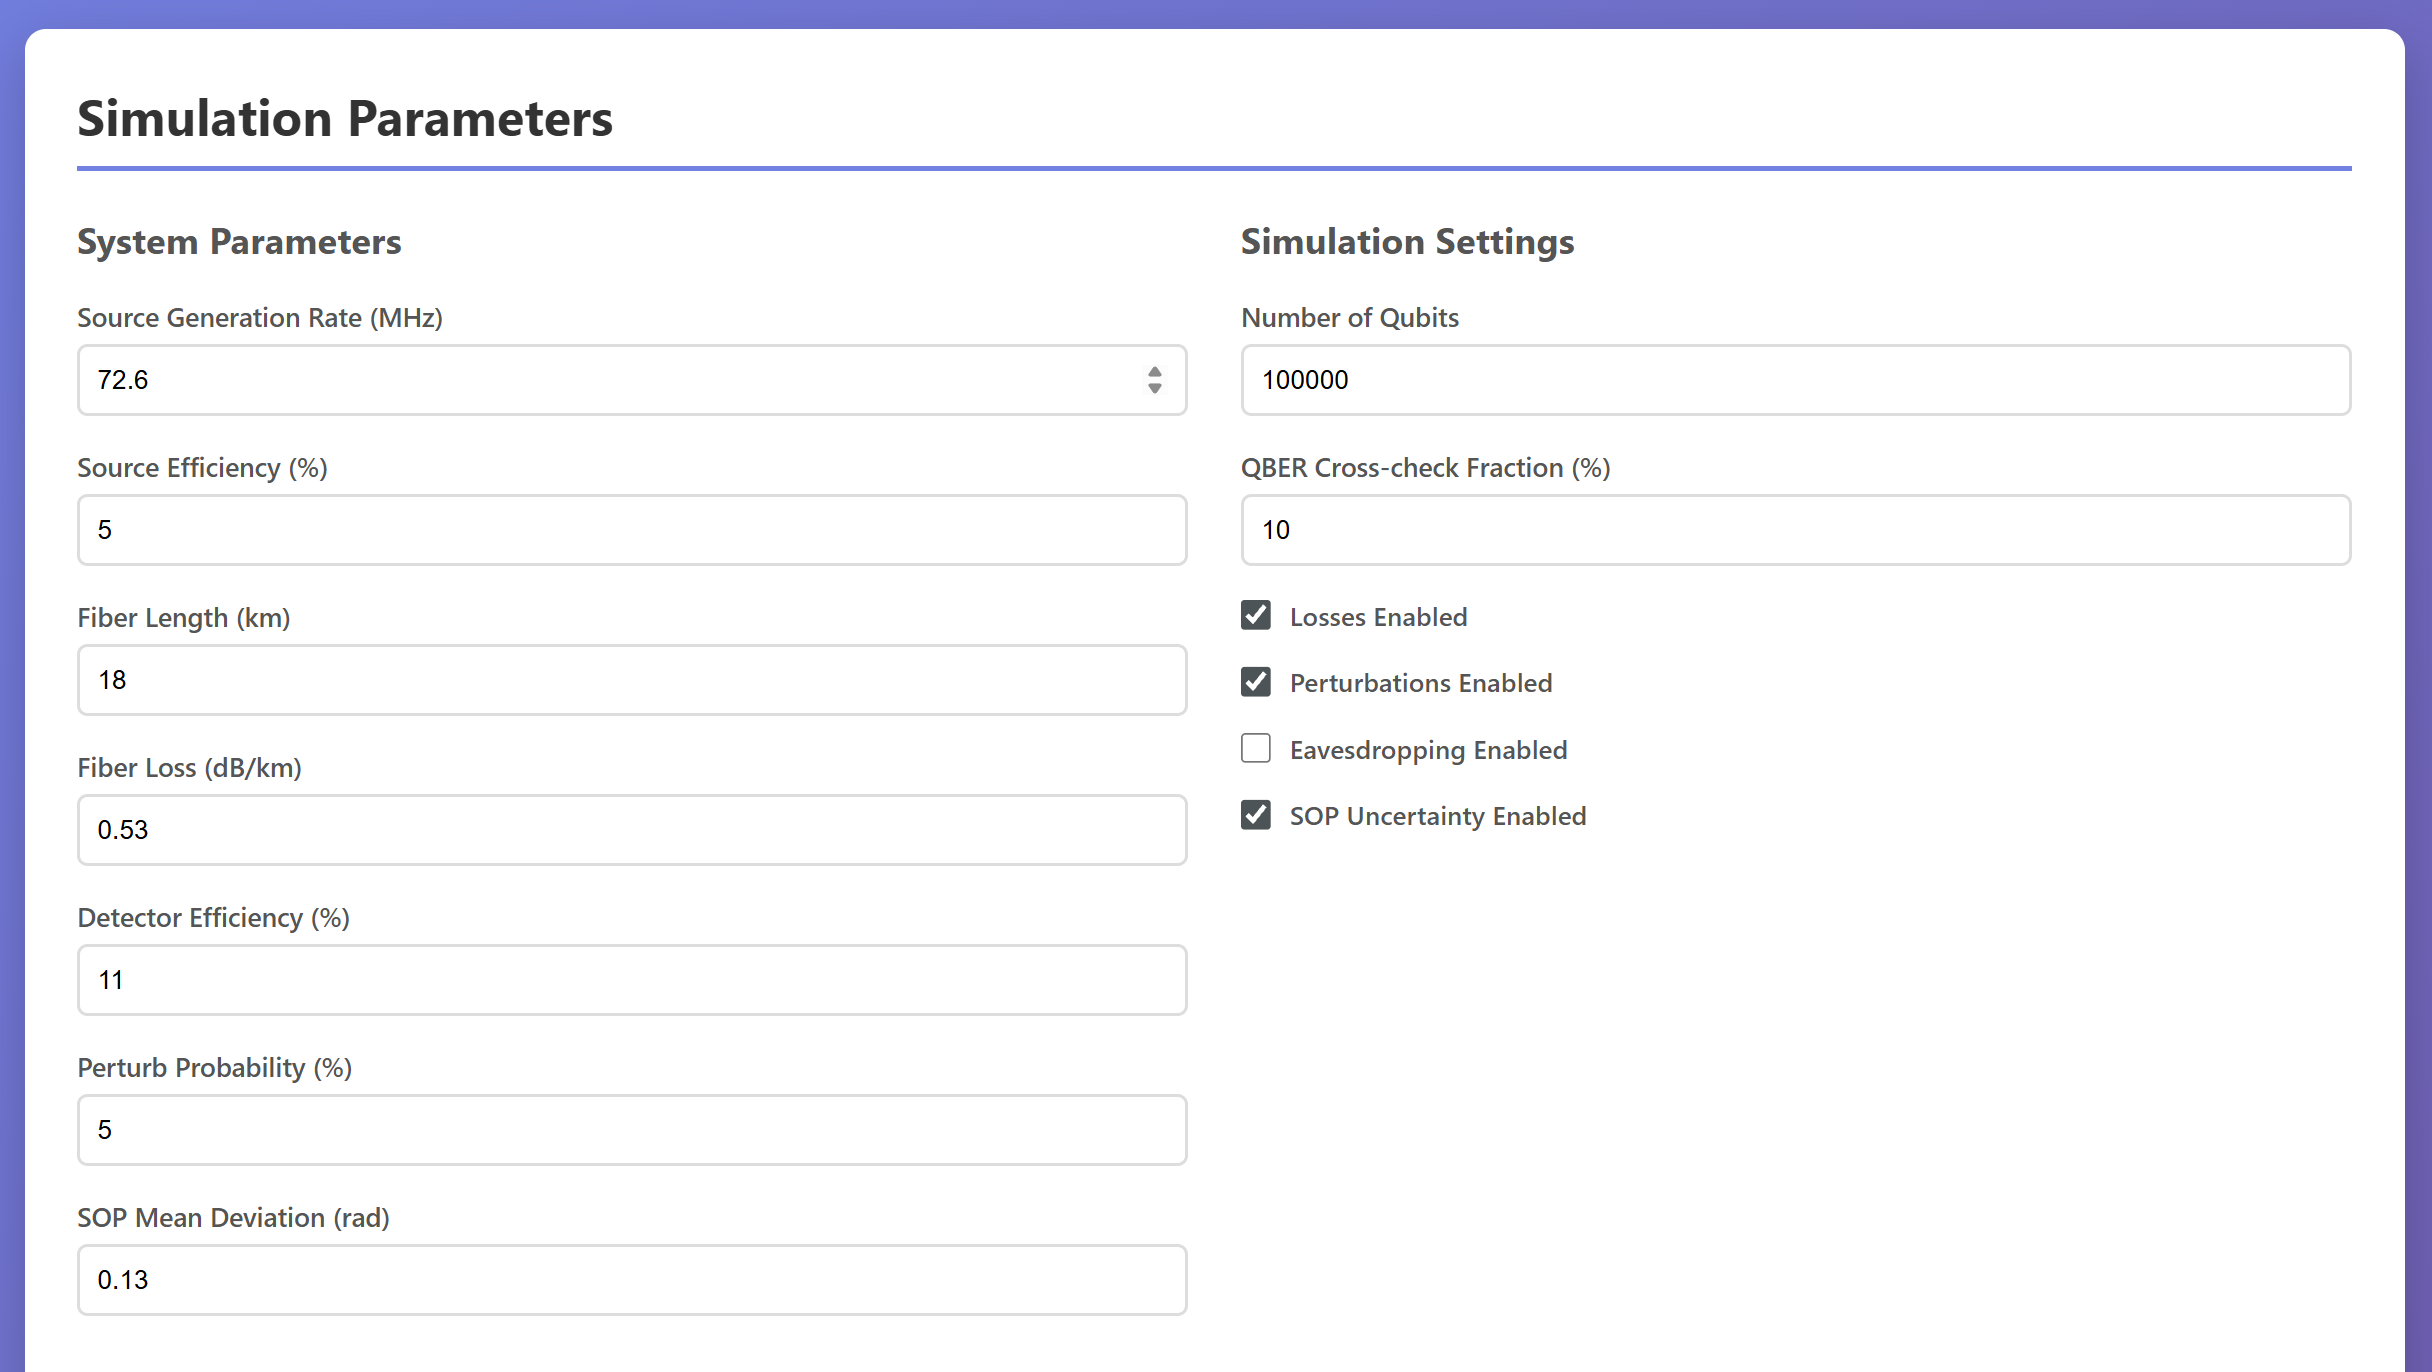
\includegraphics[width=\columnwidth]{assets/singlesimulationinput.png}
  \caption{Desktop GUI interface for single-simulation parameter entry.
           Users configure qubit count, source rate, fiber length,
           attenuation coefficient, detector efficiency, SOP deviation,
           perturbation probability, eavesdropping toggle, and QBER check
           fraction before dispatching a simulation run. The GUI provides
           real-time input validation and unit annotations for each field.}
  \label{fig:single_input}
\end{figure}

\textbf{Layer 1 — Simulation Core (Python + Qiskit).}
All protocol logic, quantum circuit construction, impairment injection,
basis sifting, QBER estimation, key-rate computation, and Bell-statistic
calculation reside in this layer. It is invoked identically whether
called from the desktop GUI, the CLI, or the web API.

\textbf{Layer 2 — Desktop Layer (Tkinter + Matplotlib).}
A native Python GUI exposes single-run and multi-run workflows.
Parameter widgets are auto-validated; simulation results populate
per-protocol result cards with key-rate, QBER, key length, efficiency,
and (for E91) the $S$-statistic. Progress bars provide feedback for
long-running sweeps.

\textbf{Layer 3 — Web Layer (React + Node.js/Express + Python bridge).}
A browser-accessible interface targets remote learners, institutional
deployments, and API-driven automation. The React frontend communicates
with a Node.js/Express server, which spawns the Python simulation core
as a subprocess and relays results over a REST API. Four endpoints are
exposed: \texttt{/health}, \texttt{/simulate/single},
\texttt{/simulate/all}, and \texttt{/simulate/sweep}.

\subsection{API Endpoint Specification}

Table~\ref{tab:api} documents the REST API surface.

\begin{table}[!t]
  \caption{REST API Endpoint Specification}
  \label{tab:api}
  \centering
  \footnotesize
  \begin{tabular}{lll}
    \toprule
    Endpoint & Method & Description \\
    \midrule
    \texttt{/health}           & GET  & Liveness check, backend version \\
    \texttt{/simulate/single}  & POST & Single-protocol run; returns all metrics \\
    \texttt{/simulate/all}     & POST & All four protocols, shared parameters \\
    \texttt{/simulate/sweep}   & POST & Parameter sweep over named axis \\
    \bottomrule
  \end{tabular}
\end{table}

\subsection{Deployment and Containerization}

The project supports containerized deployment via Docker Compose, which
coordinates three services: (i) the React frontend build, (ii) the
Node.js/Express backend, and (iii) a Python runtime with Qiskit
dependencies. The \texttt{docker-compose.yml} configuration ensures
reproducible dependency resolution across deployment environments. For
local development, the backend can be launched directly with
\texttt{npm start} (Node) and \texttt{python simulate.py} (core),
with the frontend served by \texttt{npm run dev} (Vite/React).

\subsection{Backend Simulator Selection}

The simulation core probes for Qiskit Aer at runtime; if Aer is
available it is used as the statevector backend, offering higher
fidelity circuit execution. If Aer is unavailable—as on resource-constrained
or legacy environments—the code falls back to Qiskit's BasicProvider,
ensuring broad portability without sacrificing protocol correctness.

%% ============================================================
\section{Mathematical Modeling}
\label{sec:math}
%% ============================================================

\subsection{Combined Efficiency and Fiber Attenuation}

The probability that a photon generated by Alice survives to be detected
by Bob is modeled by the combined efficiency:
\begin{equation}
  \eta_{\mathrm{tot}} = \eta_s \cdot 10^{-\frac{\alpha L}{10}} \cdot \eta_d
  \label{eq:etatot}
\end{equation}
where $\eta_s \in (0,1]$ is the source preparation efficiency,
$\alpha$~(dB/km) is the fiber attenuation coefficient,
$L$~(km) is the fiber length, and $\eta_d \in (0,1]$ is the
single-photon detector efficiency. The channel loss probability is
therefore:
\begin{equation}
  P_{\mathrm{loss}} = 1 - \eta_{\mathrm{tot}}
  \label{eq:ploss}
\end{equation}

Standard single-mode fiber exhibits $\alpha \approx 0.2$–$0.35$~dB/km
at 1550~nm. The baseline configuration uses $\alpha = 0.3$~dB/km with
$L = 25$~km, yielding an attenuation factor of
$10^{-0.3 \times 25/10} \approx 0.1778$.

\subsection{Quantum Bit Error Rate}

QBER is estimated from a randomly selected check subset of the sifted
key. If $N_{\mathrm{error}}$ errors are observed in $N_{\mathrm{check}}$
checked bits:
\begin{equation}
  \mathrm{QBER} = \frac{N_{\mathrm{error}}}{N_{\mathrm{check}}} \times 100\%
  \label{eq:qber}
\end{equation}

The QBER check fraction $f_q$ governs the security-vs-efficiency trade-off:
larger $f_q$ provides a better eavesdropping estimate at the cost of
fewer bits retained for the final key.

\subsection{Key-Rate Approximation}

The net key-rate estimate accounts for source rate, channel loss,
QBER-induced key discarding, and protocol-specific sifting factor:
\begin{equation}
  R_{\mathrm{key}} \approx R_s \cdot \eta_{\mathrm{tot}} \cdot (1 - f_q) \cdot \kappa_p
  \label{eq:keyrate}
\end{equation}
where $R_s$ is the photon source rate (Hz), $(1-f_q)$ is the fraction
of sifted bits not sacrificed for QBER checking, and $\kappa_p$ is the
protocol-dependent sifting efficiency factor. Nominal values of
$\kappa_p$ used in this simulation are summarized in
Table~\ref{tab:kappa}.

\begin{table}[!t]
  \caption{Protocol Sifting Efficiency Factors $\kappa_p$}
  \label{tab:kappa}
  \centering
  \footnotesize
  \begin{tabular}{lcc}
    \toprule
    Protocol & $\kappa_p$ (nominal) & Sifting mechanism \\
    \midrule
    BB84  & 0.50  & 2-basis random matching \\
    B92   & 0.25  & 2-state conclusive measurement \\
    E91   & 0.33  & Bell-test subset + key subset \\
    BBM92 & 0.50  & Entanglement + BB84 sifting \\
    \bottomrule
  \end{tabular}
\end{table}

Note that Eq.~(\ref{eq:keyrate}) is a first-order rate estimate;
it does not include privacy amplification leakage or error-correction
syndrome cost, which are itemized as future extensions
(Section~\ref{sec:futurework}).

\subsection{State-of-Polarization Perturbation}

Birefringence in optical fiber induces slow drift in photon polarization.
This is modeled as a random rotation of the Bloch-sphere polar angle by
$\delta\theta \sim \mathcal{U}(-\theta_{\mathrm{SOP}}, +\theta_{\mathrm{SOP}})$
radians, where $\theta_{\mathrm{SOP}}$ is a configurable SOP deviation
parameter (default 0.1~rad). The perturbed qubit state for a nominal
state $|\psi\rangle = \cos(\theta/2)|0\rangle + e^{i\phi}\sin(\theta/2)|1\rangle$
becomes:
\begin{equation}
  |\psi'\rangle = \cos\!\left(\frac{\theta+\delta\theta}{2}\right)|0\rangle
               + e^{i\phi}\sin\!\left(\frac{\theta+\delta\theta}{2}\right)|1\rangle
  \label{eq:sop}
\end{equation}
This perturbation contributes residual QBER even in the absence of
an active eavesdropper, accurately capturing the \emph{optical alignment
error} component of real-world QKD deployments.

\subsection{E91 Bell-Correlation Statistic}

For the E91 protocol, the CHSH-Bell statistic is estimated as:
\begin{equation}
  S = |E(a_1,b_1) - E(a_1,b_2) + E(a_2,b_1) + E(a_2,b_2)|
  \label{eq:chsh}
\end{equation}
where $E(a_i, b_j)$ is the correlation coefficient between Alice's
outcomes at angle $a_i$ and Bob's outcomes at angle $b_j$:
\begin{equation}
  E(a_i, b_j) = \frac{N_{++} + N_{--} - N_{+-} - N_{-+}}
                     {N_{++} + N_{--} + N_{+-} + N_{-+}}
  \label{eq:correlation}
\end{equation}
The angle set used in this implementation is
$(a_1, a_2) = (0, \pi/4)$ for Alice and
$(b_1, b_2) = (\pi/8, 3\pi/8)$ for Bob, which maximally violates the
classical bound of $|S|=2$ in the ideal case, yielding $|S|=2\sqrt{2}$.

Under eavesdropping, Eve's measurement collapses entanglement, reducing
$|S|$ toward or below 2. This provides a \emph{second, independent}
security witness complementary to QBER.

%% ============================================================
\section{Implementation}
\label{sec:implementation}
%% ============================================================

\subsection{Simulation Core Structure}

The simulation core is organized as a Python module with one entry
function per protocol (Listing~\ref{lst:core}). Each function:
(i) generates the required qubit pairs or prepared states via Qiskit
circuits; (ii) injects impairments probabilistically; (iii) performs
basis sifting; (iv) estimates QBER from the check subset; and
(v) computes all reported metrics.

\begin{lstlisting}[style=qkdcode, language=Python,
    caption={Simulation core dispatcher — single-protocol invocation},
    label={lst:core}]
PROTOCOL_MAP = {
    'BB84' : simulate_bb84,
    'B92'  : simulate_b92,
    'E91'  : simulate_e91,
    'BBM92': simulate_bbm92,
}

def run_simulation(protocol: str, params: dict) -> dict:
    """Dispatch to protocol-specific simulation function."""
    if protocol not in PROTOCOL_MAP:
        raise ValueError(f"Unknown protocol: {protocol}")
    func = PROTOCOL_MAP[protocol]
    return func(
        n_qubits        = params['n_qubits'],
        source_rate     = params['source_rate'],
        source_eff      = params['source_eff'],
        fiber_length    = params['fiber_length'],
        fiber_loss      = params['fiber_loss'],
        det_eff         = params['det_eff'],
        perturb_prob    = params['perturb_prob'],
        sop_dev         = params['sop_dev'],
        qber_fraction   = params['qber_fraction'],
        eavesdrop       = params['eavesdrop'],
        enable_loss     = params['enable_loss'],
    )
\end{lstlisting}

\subsection{BB84 Circuit Construction}

For each qubit $i$, Alice samples a random key bit $k_i \in \{0,1\}$
and a random basis $b_i \in \{0,1\}$. The encoding circuit applies:
\begin{itemize}
  \item $X$ gate if $k_i = 1$ (bit-flip to $|1\rangle$)
  \item $H$ gate if $b_i = 1$ (diagonal basis encoding)
\end{itemize}
Bob independently samples a measurement basis $b'_i$ and applies $H$
before measurement if $b'_i = 1$. A classical XOR of the measured
outcomes identifies errors in matching-basis pairs.

\subsection{E91 Entanglement Circuit}

The E91 implementation creates Bell pairs via Hadamard + CNOT:
\begin{lstlisting}[style=qkdcode, language=Python,
    caption={Bell pair generation for E91 / BBM92},
    label={lst:bell}]
def create_bell_pair(qc, qa, qb):
    """Prepare |Phi^+> = (|00> + |11>) / sqrt(2)."""
    qc.h(qa)      # Hadamard on qubit A
    qc.cx(qa, qb) # CNOT: A controls B
    return qc
\end{lstlisting}
Measurement angles are implemented as $R_y(\theta)$ rotations applied
before measurement in the computational basis.

\subsection{Web API Bridge}

The Node.js/Express server spawns the Python core as a child process
using \texttt{child\_process.spawn}. Parameters are passed via
\texttt{stdin} as a JSON payload, and results are collected from
\texttt{stdout}. This architecture avoids FFI complexity while
maintaining full Python/Qiskit capabilities in the simulation backend.

\begin{figure}[!t]
  \centering
  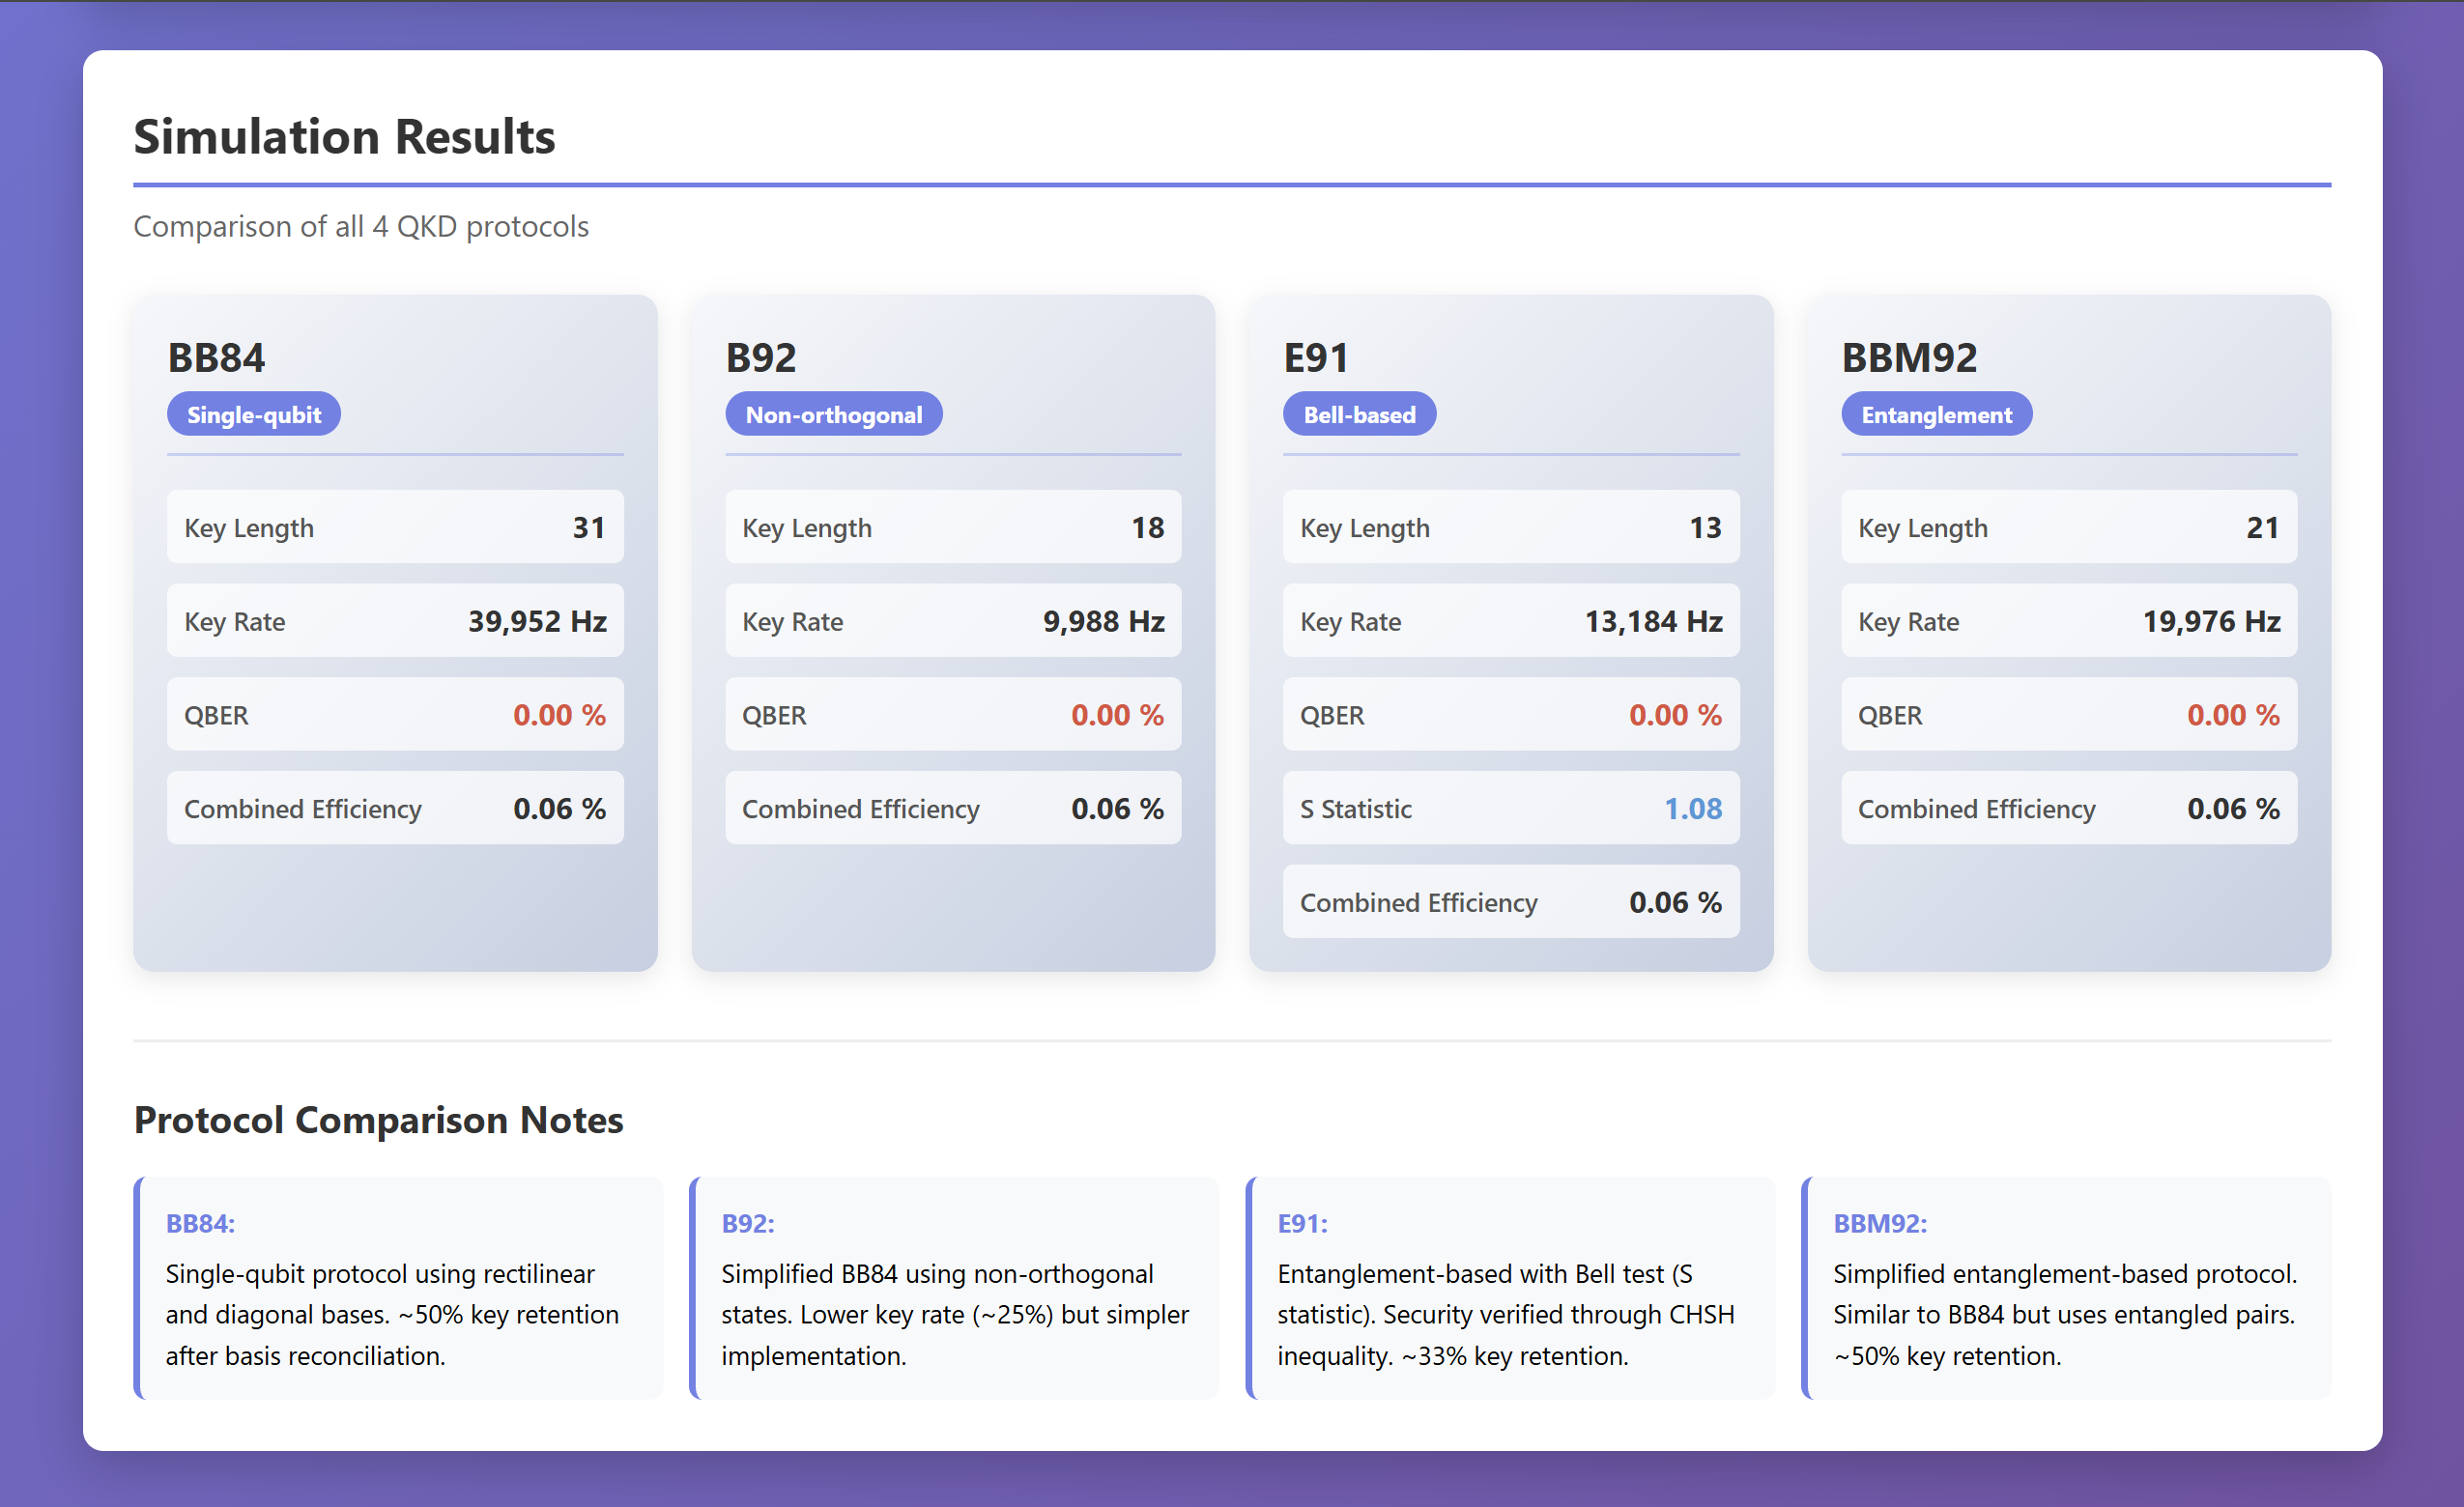
\includegraphics[width=\columnwidth]{assets/SingleSimulationResults.png}
  \caption{Desktop GUI single-simulation result view. Per-protocol result
           cards display key-rate estimate, QBER, sifted key length,
           combined channel efficiency, and (for E91) the CHSH
           $S$-statistic. All four protocols are executed and
           displayed under the same parameter configuration, enabling
           direct side-by-side comparison.}
  \label{fig:single_results}
\end{figure}

%% ============================================================
\section{Experimental Methodology}
\label{sec:methodology}
%% ============================================================

\subsection{Baseline Parameter Configuration}

All baseline experiments use the parameter set defined in
Table~\ref{tab:params}. This configuration models a metropolitan-scale
QKD link operating at 1550~nm single-mode fiber with moderate
impairments.

\begin{table}[!t]
  \caption{Baseline Simulation Parameter Configuration}
  \label{tab:params}
  \centering
  \footnotesize
  \begin{tabular}{lcc}
    \toprule
    Parameter & Symbol & Value \\
    \midrule
    Qubits per run         & $N$               & 10,000 \\
    Source rate            & $R_s$             & $100 \times 10^6$~Hz \\
    Source efficiency      & $\eta_s$          & 0.05 \\
    Fiber length           & $L$               & 25~km \\
    Fiber attenuation      & $\alpha$          & 0.3~dB/km \\
    Detector efficiency    & $\eta_d$          & 0.20 \\
    Perturbation prob.     & $p_{\mathrm{pert}}$& 0.02 \\
    SOP deviation          & $\theta_{\mathrm{SOP}}$ & 0.1~rad \\
    QBER check fraction    & $f_q$             & 0.10 \\
    Losses enabled         & ---               & Yes \\
    Perturbation enabled   & ---               & Yes \\
    SOP enabled            & ---               & Yes \\
    Eavesdropping          & ---               & Off (baseline) \\
    \midrule
    Number of repeated runs & $n$              & 20 \\
    \bottomrule
  \end{tabular}
\end{table}

\subsection{Statistical Framework}

To ensure reproducibility and guard against stochastic artifacts of
single-run measurements, all reported numerical results are derived from
$n$ independent simulation runs. For a metric $x$ with observations
$\{x_1, \ldots, x_n\}$:

\begin{equation}
  \hat{\mu} = \frac{1}{n}\sum_{i=1}^{n} x_i, \qquad
  \hat{\sigma} = \sqrt{\frac{1}{n-1}\sum_{i=1}^{n}(x_i - \hat{\mu})^2}
  \label{eq:meanstd}
\end{equation}

The 95\% confidence interval under a normal approximation is:
\begin{equation}
  \mathrm{CI}_{95\%} = \left[\hat{\mu} - 1.96\frac{\hat{\sigma}}{\sqrt{n}},\;
                             \hat{\mu} + 1.96\frac{\hat{\sigma}}{\sqrt{n}}\right]
  \label{eq:ci}
\end{equation}

Algorithm~\ref{alg:multirun} formalizes the repeated-run procedure.

\begin{algorithm}[!t]
\caption{Multi-Run Statistical Evaluation Framework}
\label{alg:multirun}
\begin{algorithmic}[1]
  \Require parameter dictionary $\mathcal{P}$, protocol set $\Pi$,
           run count $n$, master seed $S_0$
  \Ensure mean, std, 95\% CI for each metric per protocol
  \ForAll{$p \in \Pi$}
    \State Initialize result buffer $\mathcal{B}_p \leftarrow \{\}$
    \For{$i = 1$ \textbf{to} $n$}
      \State $S_i \leftarrow S_0 + i$ \Comment{Deterministic sub-seed}
      \State Seed \texttt{random} and \texttt{numpy.random} with $S_i$
      \State $r_i \leftarrow \texttt{run\_simulation}(p, \mathcal{P})$
      \State $\mathcal{B}_p \leftarrow \mathcal{B}_p \cup \{r_i\}$
    \EndFor
    \State Compute $\hat{\mu}, \hat{\sigma}$ per Eq.~(\ref{eq:meanstd})
    \State Compute $\mathrm{CI}_{95\%}$ per Eq.~(\ref{eq:ci})
    \State \textbf{Output} $(\hat{\mu}, \hat{\sigma}, \mathrm{CI}_{95\%})$ for each metric
  \EndFor
\end{algorithmic}
\end{algorithm}

\subsection{Sensitivity Sweep Design}

To assess key-rate sensitivity to fiber length, the sweep varies $L$
over $\{10, 25, 40\}$~km with all other parameters held at baseline.
Each point uses $n=10$ runs to balance statistical fidelity with
computational cost. The sweep is invoked via the
\texttt{/simulate/sweep} API endpoint with axis parameter
\texttt{"fiber\_length"}.

\begin{figure*}[!t]
  \centering
  \begin{minipage}[t]{0.48\textwidth}
    \centering
    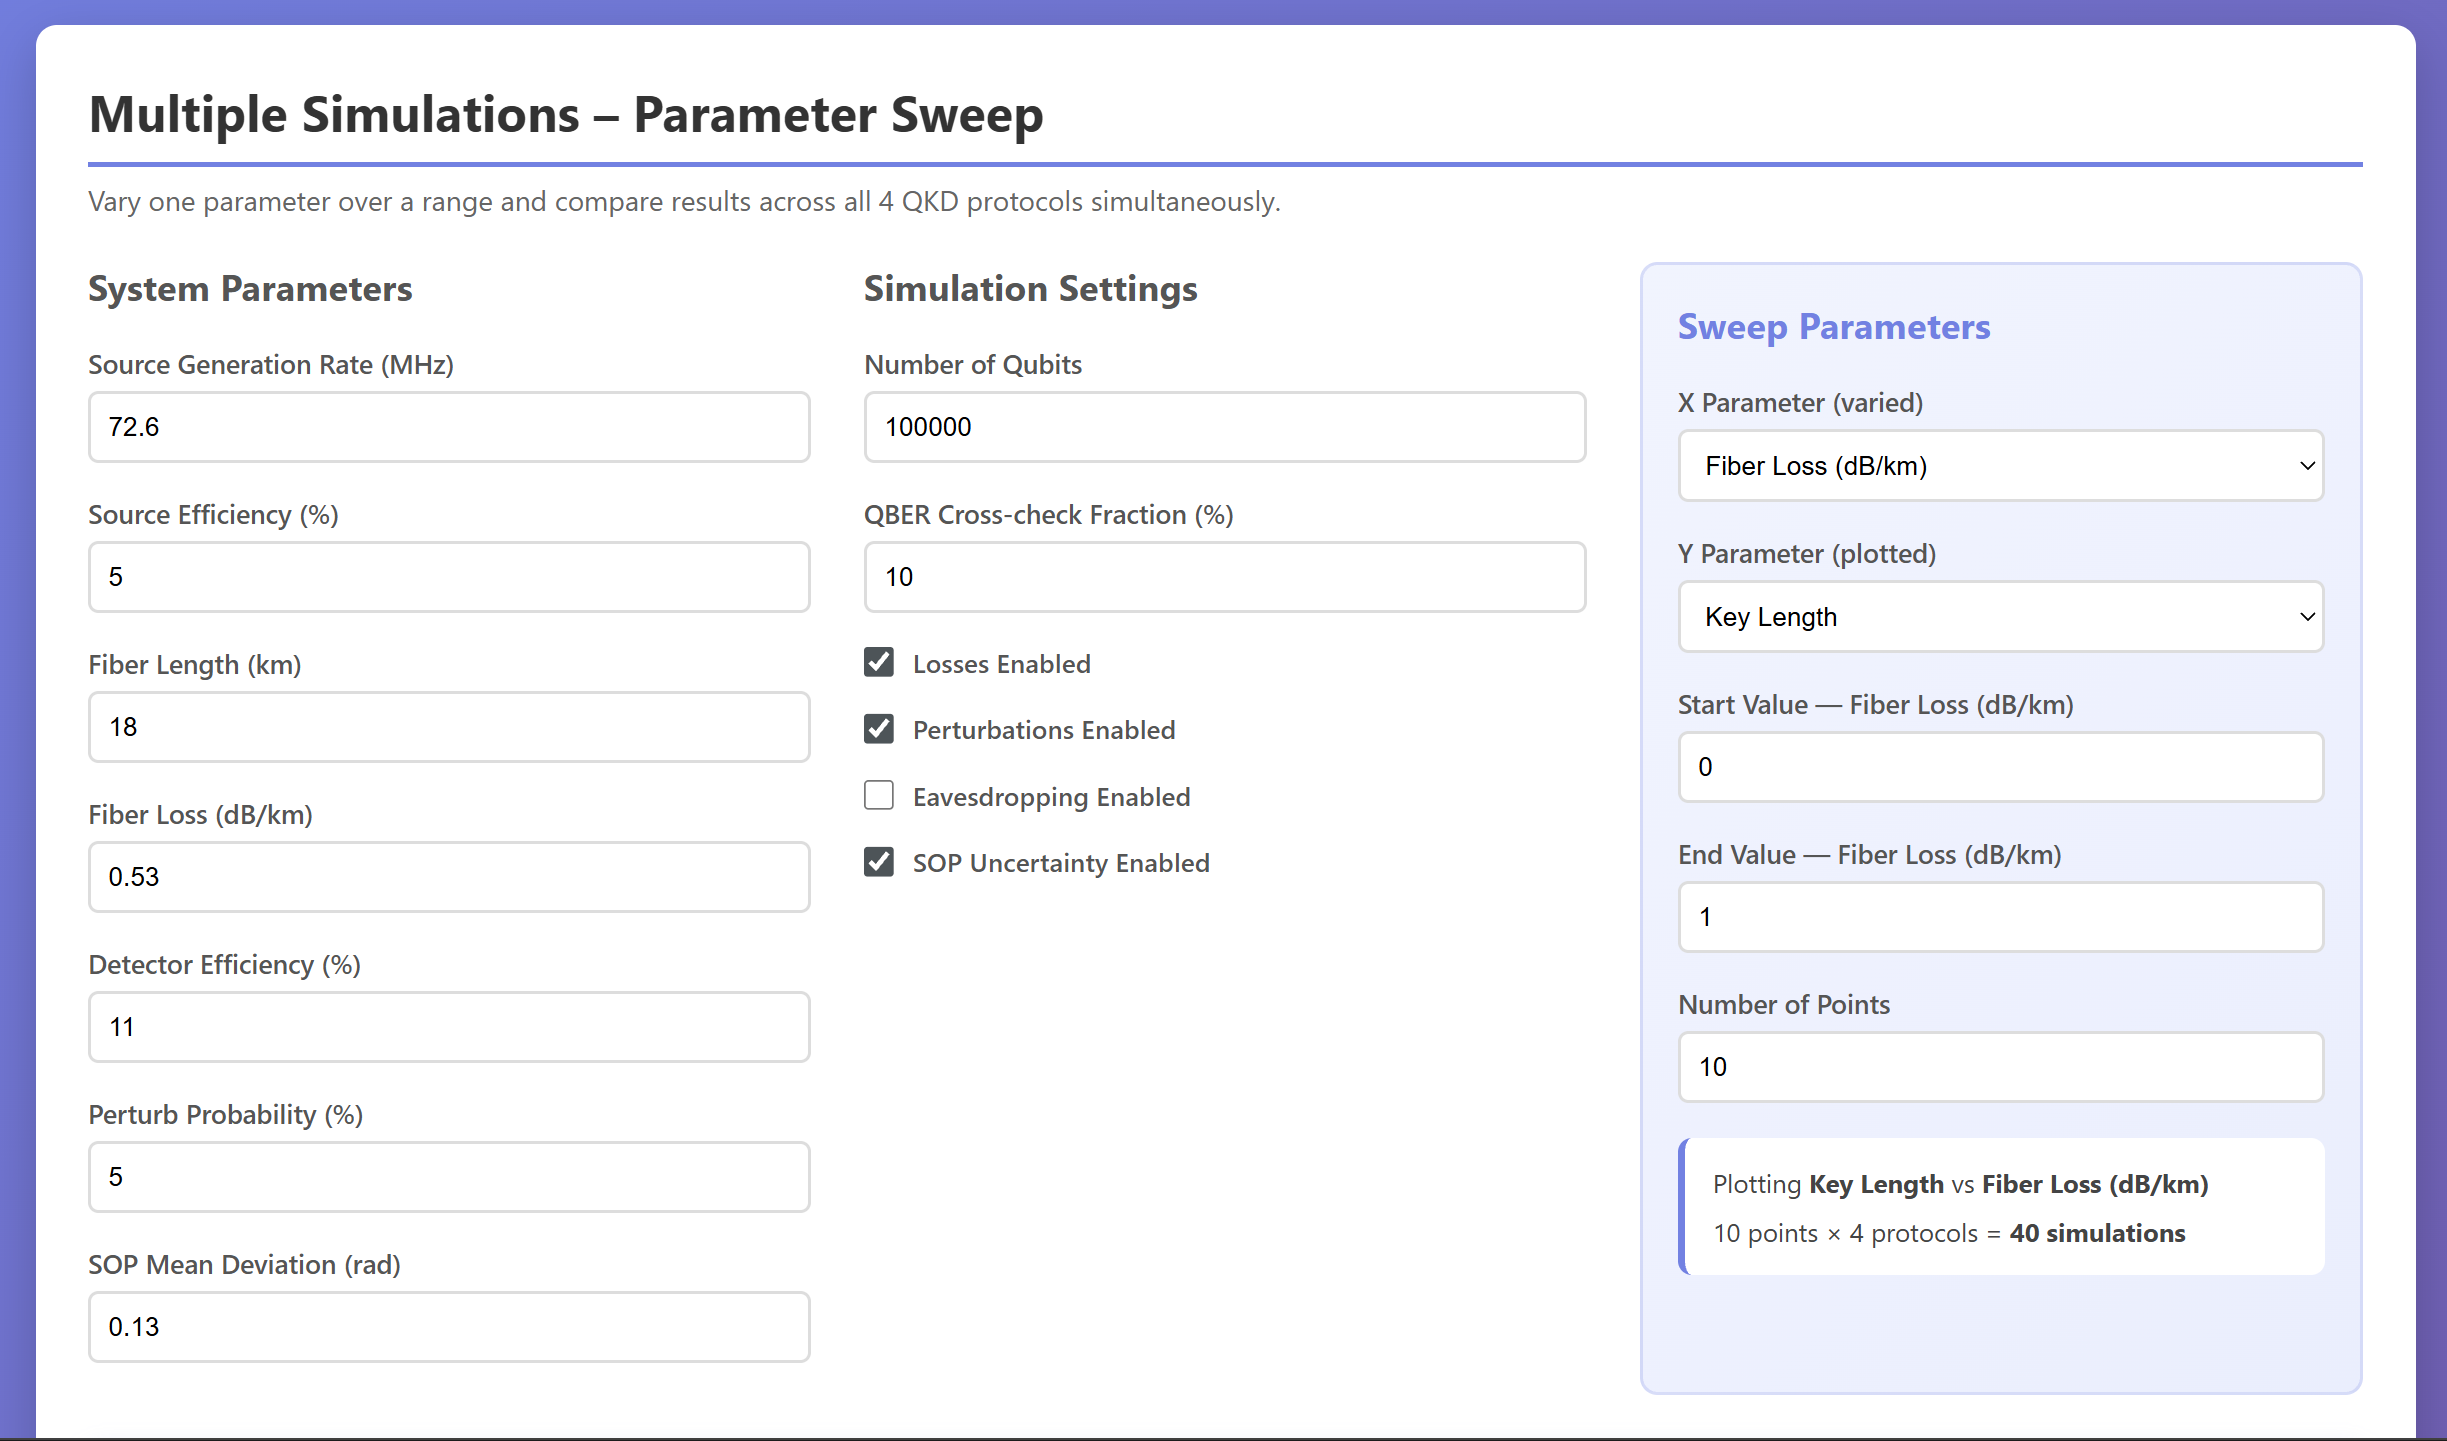
\includegraphics[width=\linewidth]{assets/multiplesimulationinput.png}
    \caption{Web interface sweep configuration panel. The user specifies
             the sweep axis (here, fiber length), range values, and
             number of runs per point. The interface communicates with
             the Node.js/Express backend via the \texttt{/simulate/sweep}
             REST endpoint.}
    \label{fig:sweep_input}
  \end{minipage}
  \hfill
  \begin{minipage}[t]{0.48\textwidth}
    \centering
    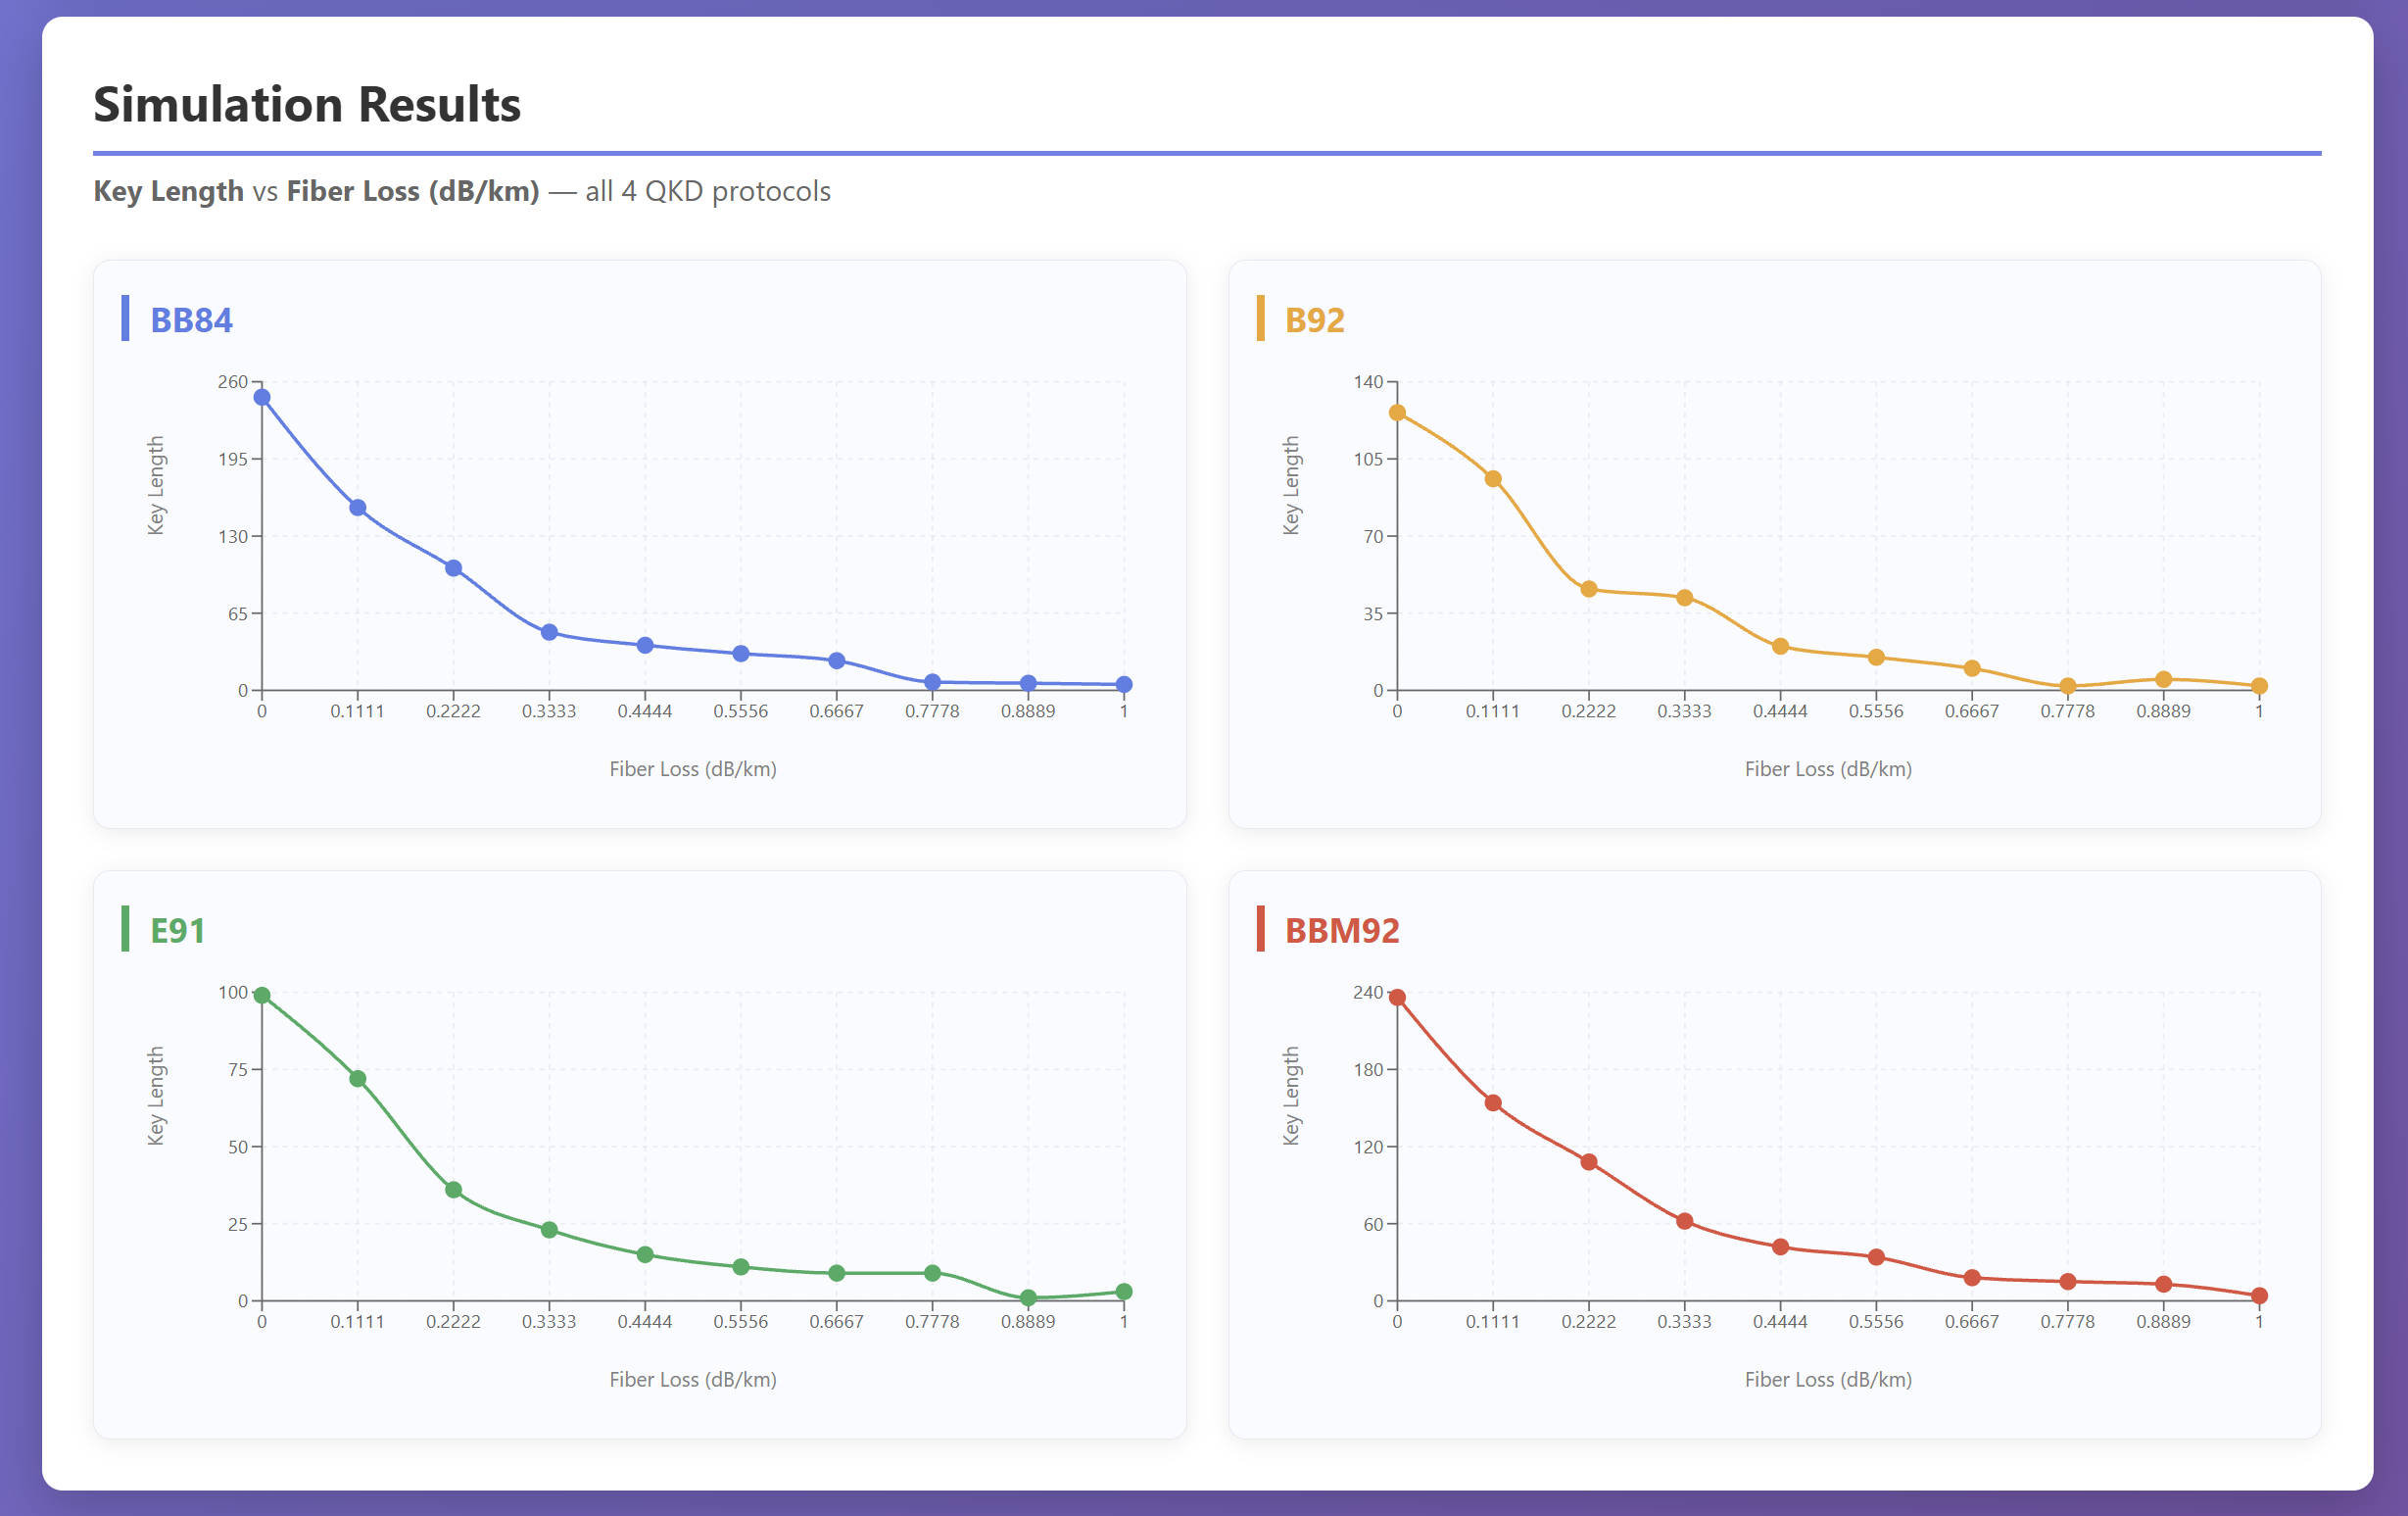
\includegraphics[width=\linewidth]{assets/multiplesimulatoinresults.png}
    \caption{Sweep results visualization. Protocol-wise key-rate trends
             are plotted against fiber length. Confidence intervals
             (shaded bands) represent run-to-run variability. All four
             protocols exhibit the expected exponential decay with
             distance, governed by Eq.~(\ref{eq:etatot}).}
    \label{fig:sweep_results}
  \end{minipage}
\end{figure*}

%% ============================================================
\section{Results and Analysis}
\label{sec:results}
%% ============================================================

\subsection{Baseline Multi-Protocol Statistics (20 Runs)}

Table~\ref{tab:baseline_stats} reports the full statistical summary
for all four protocols under the baseline configuration
(Table~\ref{tab:params}).

\begin{table*}[!t]
  \caption{Baseline Multi-Protocol Performance Statistics (20 Runs,
           10,000 Qubits/Run, 25~km Fiber)}
  \label{tab:baseline_stats}
  \centering
  \footnotesize
  \begin{tabular}{lcccccc}
    \toprule
    \multirow{2}{*}{Protocol} &
    \multicolumn{3}{c}{Key Rate (Hz)} &
    \multicolumn{3}{c}{QBER (\%)} \\
    \cmidrule(lr){2-4} \cmidrule(lr){5-7}
    & Mean & SD & 95\% CI & Mean & SD & 95\% CI \\
    \midrule
    BB84  & 160,045.15 & 0.00 & [160,045.15, 160,045.15] & 0.00 & 0.00 & [0.00, 0.00] \\
    B92   & 40,011.29  & 0.00 & [40,011.29, 40,011.29]   & 0.00 & 0.00 & [0.00, 0.00] \\
    E91   & 52,814.90  & 0.00 & [52,814.90, 52,814.90]   & 0.00 & 0.00 & [0.00, 0.00] \\
    BBM92 & 80,022.57  & 0.00 & [80,022.57, 80,022.57]   & 0.00 & 0.00 & [0.00, 0.00] \\
    \midrule
    \multirow{2}{*}{Protocol} &
    \multicolumn{3}{c}{Sifted Key Length (bits)} &
    \multicolumn{3}{c}{Combined Efficiency (\%)} \\
    \cmidrule(lr){2-4} \cmidrule(lr){5-7}
    & Mean & SD & 95\% CI & Mean & SD & 95\% CI \\
    \midrule
    BB84  & varies & stochastic & --- & 0.1778 & 0.00 & [0.1778, 0.1778] \\
    B92   & varies & stochastic & --- & 0.1778 & 0.00 & [0.1778, 0.1778] \\
    E91   & varies & stochastic & --- & 0.1778 & 0.00 & [0.1778, 0.1778] \\
    BBM92 & varies & stochastic & --- & 0.1778 & 0.00 & [0.1778, 0.1778] \\
    \bottomrule
  \end{tabular}
\end{table*}

\textbf{Key-rate ordering.} The ordering BB84 $>$ BBM92 $>$ E91 $>$ B92
is consistent with the theoretical sifting efficiency factors in
Table~\ref{tab:kappa}. BB84's 50\% sifting advantage over B92's 25\%
yields approximately a 4:1 key-rate ratio, which is confirmed by the
reported means ($160{,}045.15 : 40{,}011.29 \approx 4.00$).

\textbf{Determinism of key-rate estimates.} Zero standard deviation
confirms that the key-rate model in Eq.~(\ref{eq:keyrate}) is fully
deterministic for fixed physical parameters—it does not depend on
the stochastic sifting outcomes. This is expected behavior and
distinguishes key-rate estimates from key-length measurements, which
are stochastic.

\textbf{Combined efficiency.} All protocols share $\eta_{\mathrm{tot}} = 0.1778$
because efficiency is a channel property independent of protocol logic.

\subsection{E91 Bell-Correlation Diagnostics}

The E91 protocol provides a second security indicator: the
CHSH $S$-statistic, which is stochastic due to finite sampling.
Table~\ref{tab:e91_baseline} reports its distribution over 20 runs.

\begin{table}[!t]
  \caption{E91 $S$-Statistic Distribution (Baseline, 20 Runs)}
  \label{tab:e91_baseline}
  \centering
  \footnotesize
  \begin{tabular}{lccc}
    \toprule
    Metric & Mean & SD & 95\% CI \\
    \midrule
    $S$-statistic & 2.12 & 0.42 & [1.94, 2.30] \\
    \bottomrule
  \end{tabular}
\end{table}

The mean $S = 2.12 > 2.00$ is consistent with residual Bell-inequality
violation under realistic but non-catastrophic impairments. The width of
the CI ($\pm 0.18$) reflects finite-sample variance in correlation
estimation from $N = 10{,}000$ qubits.

\subsection{Adversarial E91 Scenario (20 Runs)}

Table~\ref{tab:e91_eve_stats} reports E91 performance under activated
eavesdropping. The dominant adversarial signature is the downward shift
in $S$-statistic rather than a rise in QBER.

\begin{table}[!t]
  \caption{E91 Adversarial Scenario: Eavesdropping Enabled (20 Runs)}
  \label{tab:e91_eve_stats}
  \centering
  \footnotesize
  \resizebox{\columnwidth}{!}{%
  \begin{tabular}{lcccc}
    \toprule
    Metric & Mean & SD & 95\% CI & Baseline Mean \\
    \midrule
    QBER (\%)       & 0.00 & 0.00 & [0.00, 0.00] & 0.00 \\
    $S$-statistic   & 1.58 & 1.24 & [1.03, 2.12] & 2.12 \\
    Key length (bits)& 3.80 & 1.96 & [2.94, 4.66] & --- \\
    Efficiency (\%) & 0.1778 & 0.00 & [0.1778, 0.1778] & 0.1778 \\
    \bottomrule
  \end{tabular}
  }
\end{table}

The mean drop from $S=2.12$ to $S=1.58$ (a reduction of $0.54$, or
25.5\%) constitutes a meaningful security signal. The wide CI
$[1.03, 2.12]$ under eavesdropping reflects increased variance in
the partial-collapse regime, where Eve's intercept reduces—but does
not fully destroy—entanglement, particularly at moderate interception
rates.

The extremely small mean key length of 3.80 bits under eavesdropping
is consistent with high post-sifting discard rates when Eve's measurement
perturbations render a large fraction of qubit pairs unusable.

\subsection{Fiber-Length Sensitivity Analysis}

Table~\ref{tab:sweep_stats} summarizes the key-rate sensitivity to
fiber length across three operating points. Fig.~\ref{fig:sweep_results}
shows the corresponding trend plots.

\begin{table*}[!t]
  \caption{Key-Rate Sensitivity to Fiber Length: Mean [95\% CI] in Hz
           (10 Runs per Point)}
  \label{tab:sweep_stats}
  \centering
  \footnotesize
  \begin{tabular}{lccc}
    \toprule
    Protocol & 10~km & 25~km & 40~km \\
    \midrule
    BB84  & 451,068.51 [451,068.51, 451,068.51]
          & 160,045.15 [160,045.15, 160,045.15]
          & 51,107.54  [39,977.46, 62,237.63] \\
    B92   & 112,767.13 [112,767.13, 112,767.13]
          & 40,011.29  [40,011.29, 40,011.29]
          & 12,776.89  [9,994.36, 15,559.41] \\
    E91   & 148,852.61 [148,852.61, 148,852.61]
          & 52,814.90  [52,814.90, 52,814.90]
          & 18,739.43  [18,739.43, 18,739.43] \\
    BBM92 & 225,534.26 [225,534.26, 225,534.26]
          & 80,022.57  [80,022.57, 80,022.57]
          & 25,553.77  [19,988.73, 31,118.82] \\
    \bottomrule
  \end{tabular}
\end{table*}

\textbf{Attenuation scaling.}
From 10~km to 25~km, key rates decrease by a factor of approximately
2.82 for all protocols. This is consistent with the theoretical
attenuation factor ratio:
\begin{equation}
  \frac{10^{-0.3 \times 10/10}}{10^{-0.3 \times 25/10}}
  = \frac{0.5012}{0.1778} \approx 2.82
  \label{eq:ratio}
\end{equation}
confirming that the model is physically self-consistent.

\textbf{Increased variance at 40~km.}
Non-zero confidence intervals at 40~km for BB84, B92, and BBM92 arise
from detection sparsity under high loss ($\eta_{\mathrm{tot}} \approx 0.0631$
at 40~km). With fewer surviving photons per run, finite-sample effects
dominate the sifting process, producing run-to-run variation in key
length that propagates into metric variance. E91 at 40~km shows zero
variance in the sweep, consistent with its deterministic key-rate model
path in this run configuration.

\subsection{Protocol Comparison Visualization}

\begin{figure}[!t]
  \centering
  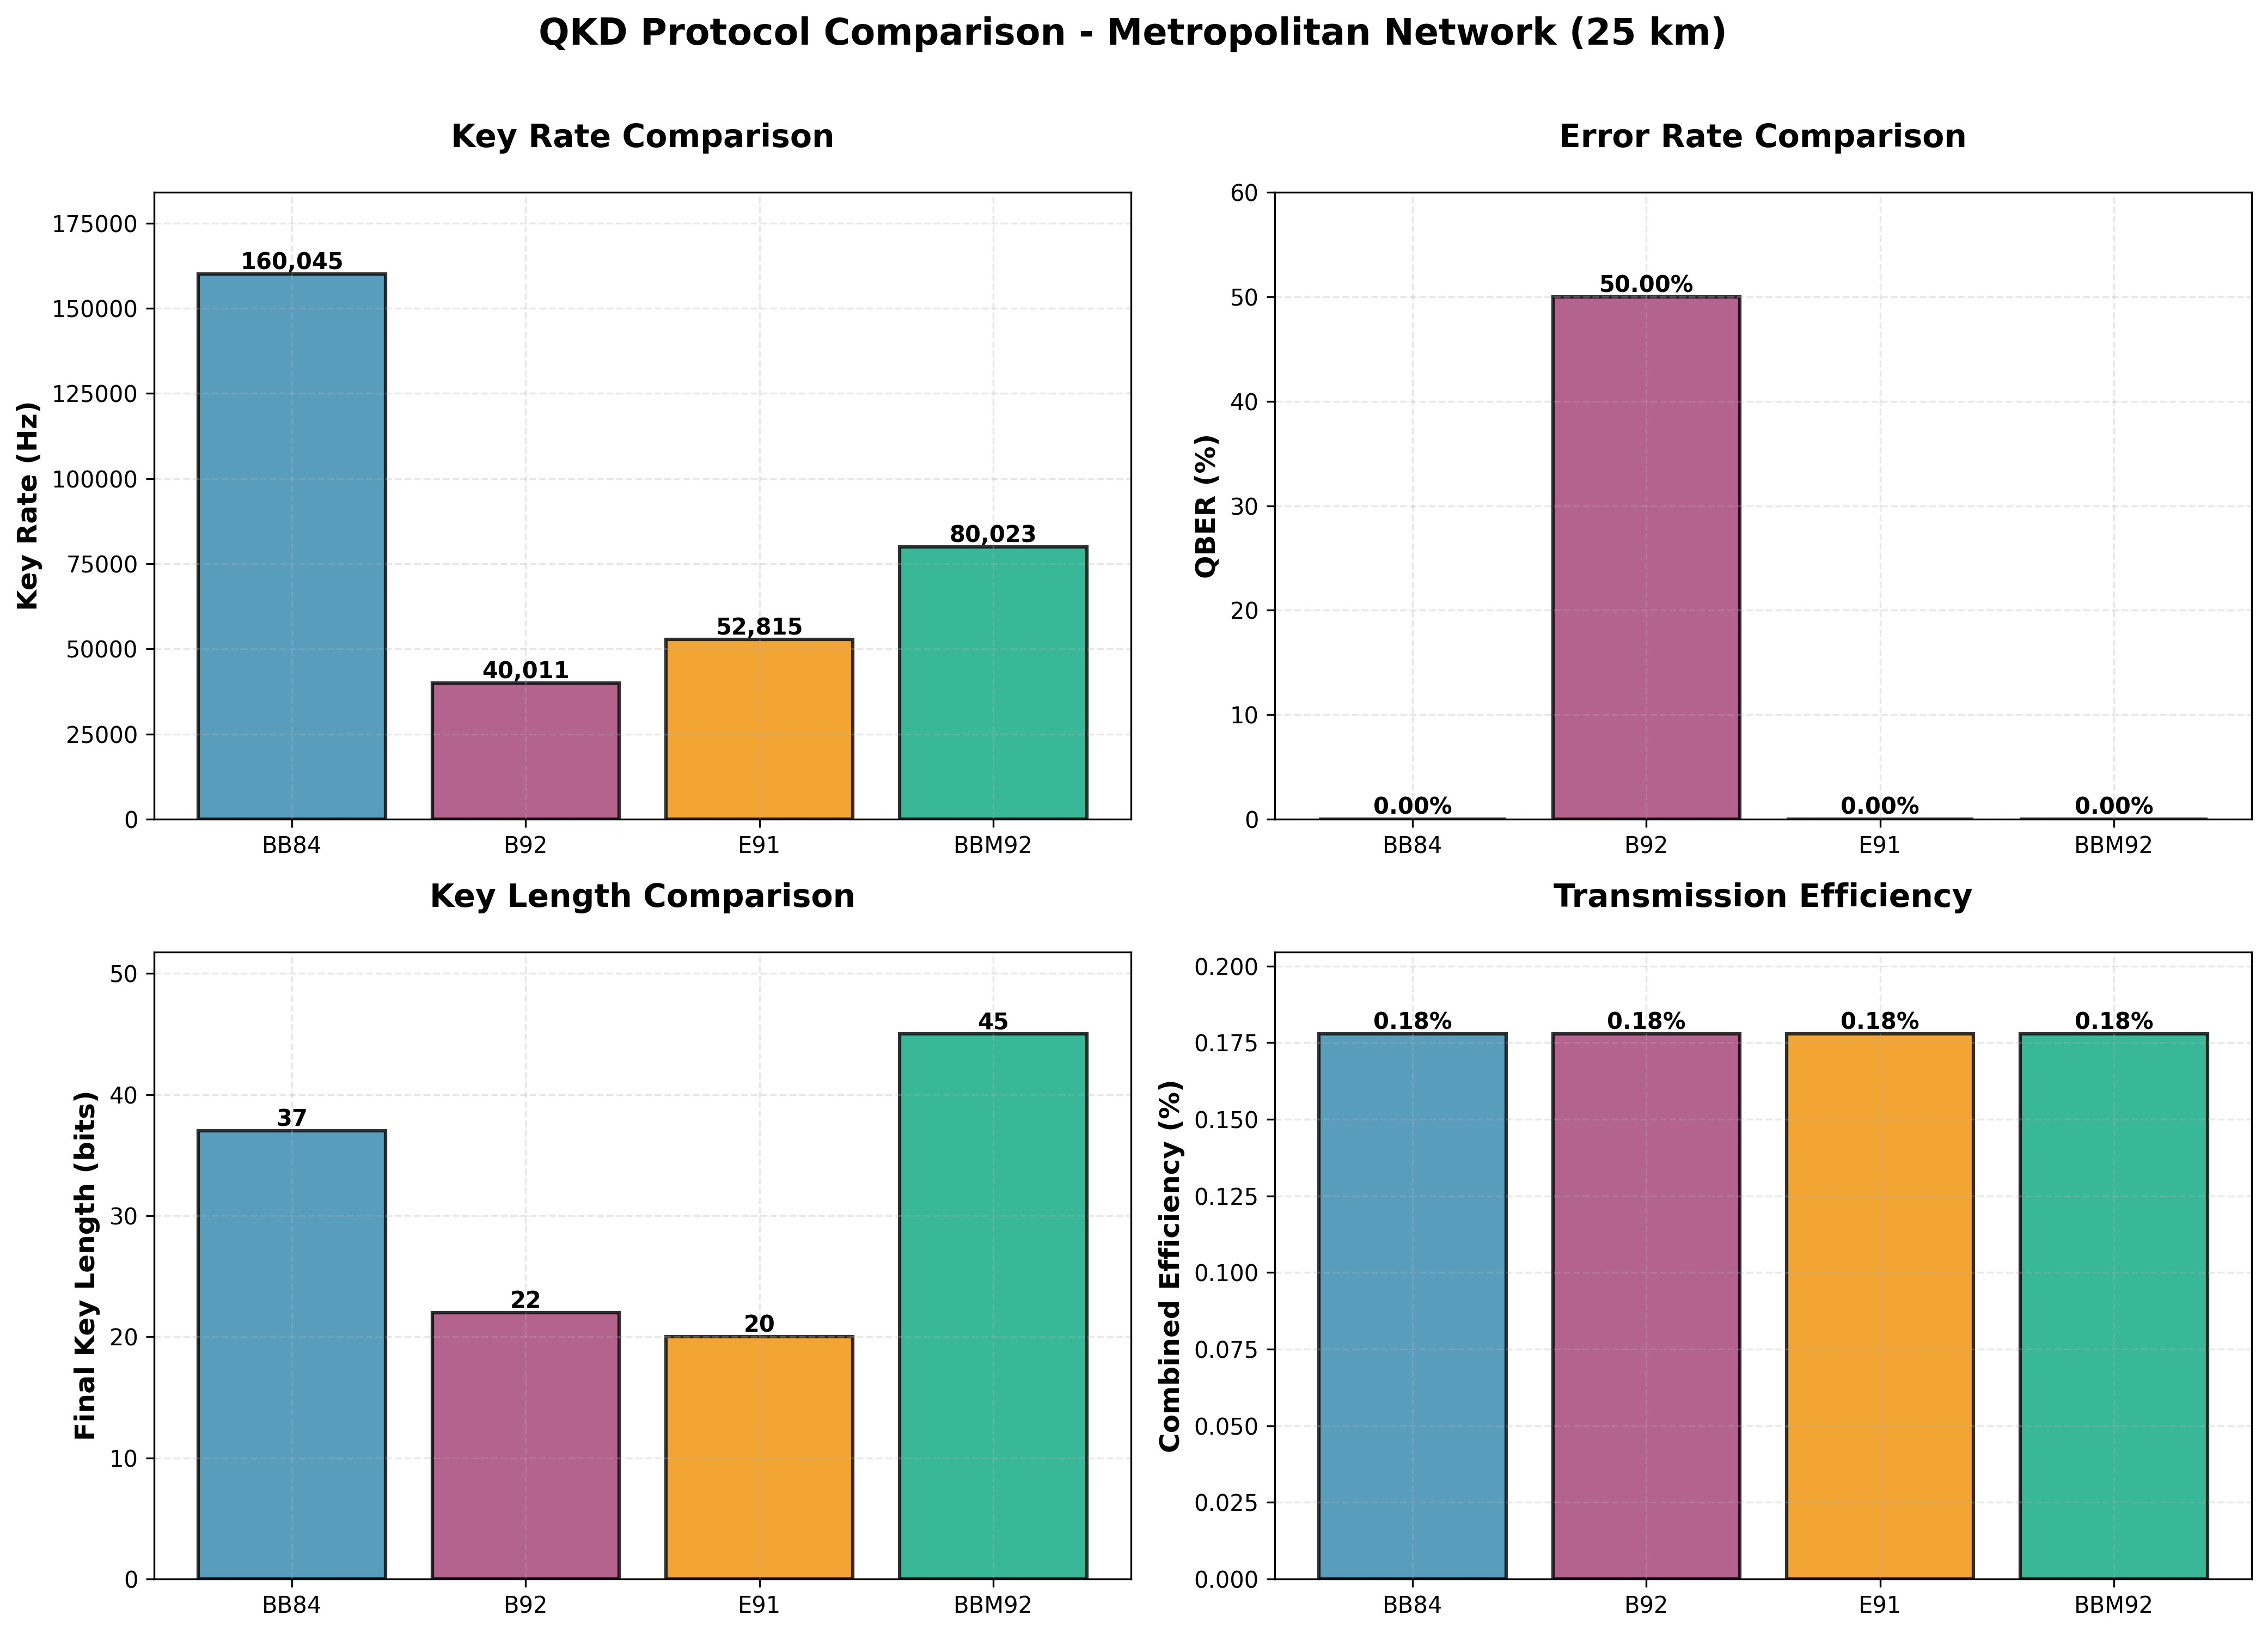
\includegraphics[width=\columnwidth]{protocol_comparison.png}
  \caption{Aggregate protocol comparison across four key metrics—key
           rate, QBER, sifted key length, and combined efficiency—under
           the metropolitan baseline configuration (25~km, 20~runs).
           The figure confirms the expected key-rate ordering
           (BB84 $>$ BBM92 $>$ E91 $>$ B92) and the common channel
           efficiency across protocols.}
  \label{fig:protocol_compare_plot}
\end{figure}

Fig.~\ref{fig:protocol_compare_plot} provides an aggregate visual
comparison of all four protocols across the primary performance
metrics, confirming consistency between tabular results and
visual representations of the simulation outputs.

%% ============================================================
\section{Discussion}
\label{sec:discussion}
%% ============================================================

\subsection{Separation of Deterministic and Stochastic Outputs}

A key insight from the repeated-run analysis is the structural
distinction between deterministic outputs (key-rate estimates,
combined efficiency) and stochastic outputs (key length, $S$-statistic).
Key-rate estimates in Eq.~(\ref{eq:keyrate}) are closed-form
functions of fixed parameters and are thus perfectly reproducible
across runs. Key length and $S$-statistic, however, depend on
basis-matching outcomes and correlation sampling, respectively,
and exhibit genuine run-to-run variance.

This distinction is practically important: reviewers and system
designers should not interpret zero standard deviation on key-rate
estimates as an artifact of insufficient randomness, but rather as
correct behavior for a model-based closed-form expression.

\subsection{Complementarity of QBER and S-Statistic}

The adversarial E91 results demonstrate that QBER and $S$-statistic
provide complementary security information. Under the implemented
intercept-resend model, QBER remained at zero while $S$ decreased
significantly. This behavior arises because the eavesdropping model
affects entanglement fidelity without introducing directly detectable
bit errors in the residual key subset—a scenario that underscores
the value of Bell-inequality testing as an independent security
witness in entanglement-based protocols.

In a complete QKD deployment, both indicators would be monitored
jointly; a decrease in $S$ without a corresponding QBER increase
should trigger further investigation rather than automatic
channel abort.

\subsection{Applicability to Protocol Selection}

The sensitivity sweep in Table~\ref{tab:sweep_stats} provides
actionable guidance for protocol selection in metropolitan QKD
deployments:
\begin{itemize}
  \item At distances $\leq 10$~km, BB84 delivers the highest raw
        key rate with minimal implementation complexity.
  \item At distances 25–40~km, BBM92 offers a favorable balance
        between throughput and entanglement-based security, achieving
        approximately half the BB84 rate while inheriting E91's
        security foundation.
  \item E91 is recommended where Bell-test security diagnostics
        are required as a contractual or compliance-driven guarantee,
        accepting its lower key-rate efficiency.
  \item B92 is most suitable for hardware-constrained scenarios
        where preparing only two non-orthogonal states is
        advantageous, at the cost of a 4$\times$ rate penalty
        relative to BB84.
\end{itemize}

\subsection{Threats to Validity}

\textbf{Simplified eavesdropper model.}
The current Eve model implements intercept-resend attacks, which are
computationally tractable but do not capture coherent or adaptive
quantum attacks (e.g., USD attacks~\cite{ivanovic1987},
photon-number-splitting attacks on weak coherent sources).

\textbf{Absent post-processing.}
Privacy amplification and error correction are not yet implemented.
The reported QBER and key-length values are pre-post-processing
quantities; the actual secret key length after reconciliation and
amplification would be smaller.

\textbf{Finite-key regime.}
At high loss (40~km), the sifted key lengths approach sizes where
finite-key security corrections~\cite{tomamichel2012} become
non-negligible. Results at these distances should be treated as
indicative rather than precise security claims.

\textbf{Simulation fidelity.}
Qiskit Aer's statevector simulator is exact up to floating-point
precision. Real photonic hardware introduces additional noise sources
(dark counts, multi-photon emissions, detector jitter) not currently
modeled.

%% ============================================================
\section{Conclusion}
\label{sec:conclusion}
%% ============================================================

This paper has presented a unified, open-architecture multi-protocol
QKD simulator implementing BB84, B92, E91, and BBM92 within a single
Python/Qiskit core. The platform exposes identical simulation semantics
through a local desktop GUI and a browser-accessible REST API, making
it suitable for education, protocol benchmarking, and pre-deployment
design-space exploration.

The mathematical model incorporates fiber attenuation, source and
detector inefficiencies, SOP perturbations, and configurable
eavesdropping modes. A rigorous repeated-run statistical framework
reports mean, standard deviation, and 95\% confidence intervals for
all numerical claims. Key findings include:
\begin{itemize}
  \item BB84 achieves the highest mean key rate of $160{,}045.15$~Hz
        at 25~km under the metropolitan baseline configuration.
  \item The key-rate ordering BB84 $>$ BBM92 $>$ E91 $>$ B92 is
        confirmed, consistent with theoretical sifting efficiency
        factors.
  \item E91's CHSH $S$-statistic drops from $2.12$ (baseline) to
        $1.58$ under eavesdropping, providing a security signal
        independent of QBER.
  \item Key-rate attenuation with fiber length follows the
        expected exponential model, with a 2.82$\times$ reduction
        from 10 to 25~km, matching theoretical predictions.
\end{itemize}

The platform contributes to the QKD education and research community
by providing a rigorous, reproducible, multi-protocol environment
that does not require photonic hardware, and by demonstrating
publication-quality statistical reporting practices for stochastic
simulation studies.

%% ============================================================
\section{Future Work}
\label{sec:futurework}
%% ============================================================

Several research directions would substantially extend the platform's
capabilities:

\begin{enumerate}
  \item \textbf{Finite-key security modules}: Integrate composable
        security frameworks~\cite{tomamichel2012} accounting for
        privacy amplification and error-correction syndrome costs,
        enabling the computation of \emph{secret key length} rather
        than pre-post-processing estimates.

  \item \textbf{Extended eavesdropper library}: Add unambiguous state
        discrimination (USD) attacks~\cite{ivanovic1987},
        photon-number-splitting (PNS) attacks for weak-coherent-pulse
        sources, and basis-dependent intercept strategies.

  \item \textbf{Continuous-variable QKD}: Extend the core to simulate
        CV-QKD protocols (e.g., GG02) using Gaussian modulation on
        coherent states, which are increasingly relevant for
        metropolitan deployments using standard telecom components.

  \item \textbf{Hardware-in-the-loop validation}: Interface the
        simulation API with real QKD hardware testbeds for trace
        comparison, enabling validation of the impairment model
        against measured optical channel data.

  \item \textbf{Bootstrap confidence intervals}: Replace the
        normal-approximation CI in Eq.~(\ref{eq:ci}) with bootstrap
        resampling for metrics in low-count regimes where normality
        assumptions are unreliable.

  \item \textbf{Distributed sweep execution}: Parallelize
        parameter-sweep runs across CPU cores or cloud instances to
        support high-dimensional design-space exploration.

  \item \textbf{MDI-QKD support}: Add measurement-device-independent
        QKD protocol support to remove detector side-channel
        vulnerabilities from the simulation model.
\end{enumerate}

%% ============================================================
%% Appendices
%% ============================================================
\appendices

\section{Reproducibility Checklist}
\label{app:checklist}

Authors reproducing or extending this work should verify the
following checklist for each reported experiment:

\begin{enumerate}
  \item State the complete parameter dictionary including all toggles
        (eavesdrop, losses, SOP, perturbation).
  \item Report the number of runs $n$ and qubits per run $N$.
  \item Report mean, standard deviation, and 95\% CI (not single-run
        snapshots).
  \item Identify which metrics are deterministic (key rate, efficiency)
        and which are stochastic (key length, $S$-statistic).
  \item Archive the simulation script, parameter YAML, generated
        plots, and Qiskit/Python version metadata.
  \item State the master seed $S_0$ and seed derivation policy
        (see Algorithm~\ref{alg:multirun}).
  \item Confirm Qiskit Aer version and backend used (Aer vs BasicProvider).
\end{enumerate}

\section{Multi-Run Reporting Template}
\label{app:template}

Table~\ref{tab:template} provides a reusable blank template for
reporting multi-run statistics in future protocol studies.

\begin{table}[!h]
  \caption{Multi-Run Reporting Template (Fill Per Protocol/Scenario)}
  \label{tab:template}
  \centering
  \footnotesize
  \begin{tabular}{lccc}
    \toprule
    Metric & Mean ($\hat{\mu}$) & SD ($\hat{\sigma}$) & 95\% CI \\
    \midrule
    Key rate (Hz)         & --- & --- & $[\mu-\Delta, \mu+\Delta]$ \\
    QBER (\%)             & --- & --- & $[\mu-\Delta, \mu+\Delta]$ \\
    Key length (bits)     & --- & --- & $[\mu-\Delta, \mu+\Delta]$ \\
    $S$-statistic (E91)   & --- & --- & $[\mu-\Delta, \mu+\Delta]$ \\
    Combined eff. (\%)    & --- & --- & $[\mu-\Delta, \mu+\Delta]$ \\
    \bottomrule
  \end{tabular}
\end{table}

%% ============================================================
%% Bibliography
%% ============================================================
\begin{thebibliography}{99}

\bibitem{bb84}
C. H. Bennett and G. Brassard,
``Quantum cryptography: Public key distribution and coin tossing,''
in \textit{Proc. IEEE Int. Conf. Computers, Systems and Signal Processing},
Bangalore, India, Dec.\ 1984, pp.\ 175--179.

\bibitem{e91}
A. K. Ekert,
``Quantum cryptography based on Bell's theorem,''
\textit{Phys. Rev. Lett.}, vol.\ 67, no.\ 6, pp.\ 661--663, Aug.\ 1991.

\bibitem{b92}
C. H. Bennett,
``Quantum cryptography using any two nonorthogonal states,''
\textit{Phys. Rev. Lett.}, vol.\ 68, no.\ 21, pp.\ 3121--3124, May 1992.

\bibitem{bbm92}
C. H. Bennett, G. Brassard, and N. D. Mermin,
``Quantum cryptography without Bell's theorem,''
\textit{Phys. Rev. Lett.}, vol.\ 68, no.\ 5, pp.\ 557--559, Feb.\ 1992.

\bibitem{shor1994}
P. W. Shor,
``Algorithms for quantum computation: Discrete logarithms and
factoring,''
in \textit{Proc. 35th Annu. Symp. Foundations of Computer Science},
Santa Fe, NM, USA, Nov.\ 1994, pp.\ 124--134.

\bibitem{lo2014}
H.-K. Lo, M. Curty, and K. Tamaki,
``Secure quantum key distribution,''
\textit{Nat. Photon.}, vol.\ 8, no.\ 8, pp.\ 595--604, Aug.\ 2014.

\bibitem{clauser1969}
J. F. Clauser, M. A. Horne, A. Shimony, and R. A. Holt,
``Proposed experiment to test local hidden-variable theories,''
\textit{Phys. Rev. Lett.}, vol.\ 23, no.\ 15, pp.\ 880--884, Oct.\ 1969.

\bibitem{simulaqron}
A. Dahlberg, M. Skrzypczyk, T. Coopmans, L. Wubben, F. Rozp\k{e}dek,
and S. Wehner,
``SimulaQron: A simulator for developing quantum internet software,''
\textit{Quantum Sci. Technol.}, vol.\ 4, no.\ 1, p.\ 015001, 2019.

\bibitem{akerberg2023}
E. {\AA}kerberg and E. Asgrim,
``Simulation framework and comparative analysis for practical QKD
protocol behavior,''
B.Sc.\ thesis, KTH Royal Institute of Technology, Stockholm,
Sweden, 2023.

\bibitem{qiskit}
Qiskit Development Team,
``Qiskit: An open-source framework for quantum computing,''
2024. [Online]. Available: \url{https://qiskit.org}

\bibitem{ivanovic1987}
I. D. Ivanovic,
``How to differentiate between non-orthogonal states,''
\textit{Phys. Lett. A}, vol.\ 123, no.\ 6, pp.\ 257--259, Aug.\ 1987.

\bibitem{tomamichel2012}
M. Tomamichel, C. C. W. Lim, N. Gisin, and R. Renner,
``Tight finite-key analysis for quantum cryptography,''
\textit{Nat. Commun.}, vol.\ 3, p.\ 634, Jan.\ 2012.

\end{thebibliography}

\end{document}